\section{Présentation du projet}

\subsection{Présentation de notre modèle}

\subsubsection{Les différentes bases}

Pour notre projet, nous avons décidé de fédérer deux bases de données hétérogènes : une base de données relationnelles et une base de données XML. Les données présentes dans ces bases modélisent des pokémons. Les pokémons sont des monstres issus de la culture japonaise. Ces pokémons possèdent un ou plusieurs types (feu, eau, plante…) et des compétences. Ils sont possédés par des dresseurs. Ces dresseurs forment des équipes. Une description plus complète de ce contexte est faite en annexe A.

La base SQL possède une table synthétisant certaines des caractéristiques des pokémons.
\begin{itemize}
\item id : identifiant du pokémon	
\item name : nom du pokémon	
\item height, weight : taille et poids du pokémon	
\item base\_experience : base servant à calculer, après application de coefficients, le gain réel d'expérience
\end{itemize}

\begin{tabular}{|c|c|c|c|c|}
 \hline
 id & name & height & weight & base\_experience \\
 \hline
\end{tabular}

La seconde base de données, la base XML, dispose de 3 fichiers XML : pokémons.xml, teams.xml et moves.xml. Le fichier pokémons.xml regroupe le ou les types de chaque pokémon. Le fichier teams.xml regroupe toutes les teams. Une team est composée d'un dresseur de pokémons. Ce fichier permet de savoir quels pokémons possédait chaque team. Enfin le fichier moves.xml regroupe tous les moves existants, c'est-à-dire toutes les compétences que peuvent avoir les pokémons.

 \subsubsection{Schéma externe}

Du point de vue de l'utilisateur, les données issues des différentes bases sont regroupées sous un même modèle appelé schéma externe. Lorsque le client veut accéder à des données, il effectue une requête sur ce modèle. La réponse qu'il obtiendra respectera également le modèle du schéma externe.

Le schéma externe est représenté par le fichier xsd présent en Annexe B.

\subsection{Implémentation de la base de données fédérée}

Pour implémenter notre projet, nous avons choisi d'utiliser le langage de script Python version 3.3 car ce dernier offre une grande flexibilité grâce à diverses librairies et une grande simplicité de code. Les principales librairies utilisées pour notre projet sont :

\begin{itemize}
    \item zorba : processeur qui permet d'effectuer des requêtes XQuery ;

    \item sqlite3 : librairie qui permet de faire des requêtes SQL sur une base SQLite ;

    \item xml.eTree : permet la manipulation de fichier XML et d'objet XML en Python (création, édition, etc.).
\end{itemize}

Chaque fonctionnalité est codée dans un fichier portant le nom de la fonctionnalité implémentée.

\begin{figure}[h!]
    \centering
    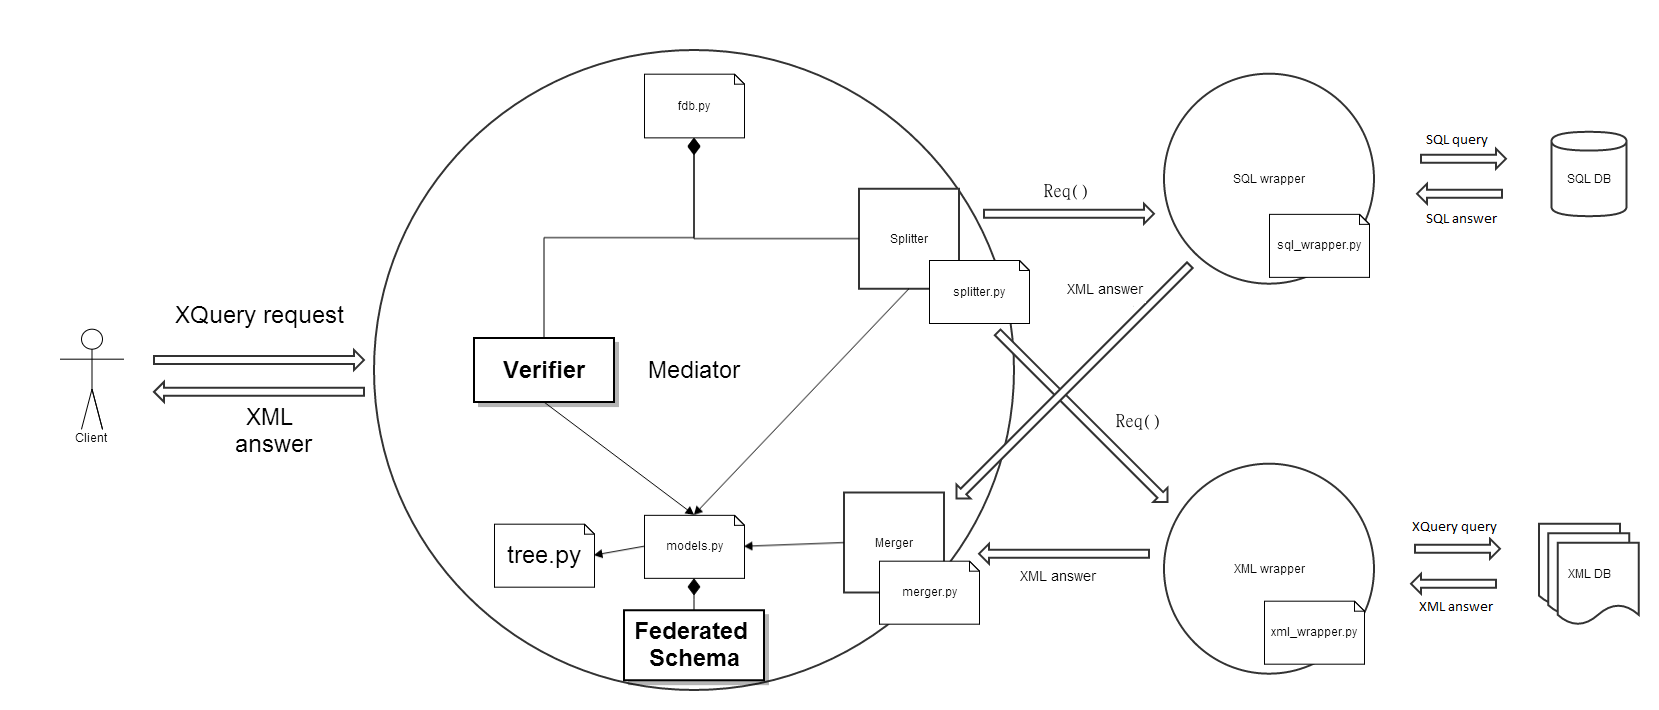
\includegraphics[width=1\textwidth]{ressources/graphiques/architecture.png}
    \caption{Schéma général de l'architecture du projet}
\end{figure}

Le client, souhaitant interroger son système d'information, lance une requête XQuery. Cette requête ne prend pas en compte la totalité de la syntaxe XQuery mais une limitation assez basique de cette dernière : l'utilisateur peut uniquement effectuer des "for … where … return …" et les requêtes imbriquées ne sont pas gérées. De plus les conditions sont triviales avec toujours un couple variable/valeur (par exemple, $where \$var <> "valeur"$). Pour ce qui est du return, il renverra tout le temps la variable définie dans le for.

\subsubsection{Verifier}

La requête passe en premier lieu par le "Verifier". Ce dernier a pour rôle de contrôler la requête, c'est-à-dire vérifier la syntaxe. Cette vérification est autant lexicale, que syntaxique, puisqu'il s'agit notamment de vérifier que la requête se limite bien à la syntaxe proposée. La vérification possède également un aspect sémantique, et en particulier, le "Verifier" certifie que les noms des tables utilisés sont reconnus. Si le "Verifier" valide la requête, cette dernière est envoyée au "Splitter".

\subsubsection{Splitter}

Le "Splitter" doit séparer la requête en autant de sous-requêtes qu'il faut faire dans les sous-bases. Une sous-requête correspond à la lecture d'une table SQL ou d'un fichier XML. 

Nous allons illustrer son fonctionnement. Prenons l'exemple suivant de requête XQuery :

\begin{lstlisting}
for $type in doc()//team[victory > 10]/pokemon/type1
where $type <> "Grass"
return $type
\end{lstlisting}

La partie for sera analysée et divisée selon son contenu. On se concentre seulement sur la partie xPath de l'expression :
\begin{lstlisting}
//team[victory > 10]/pokemon/type1
\end{lstlisting}
On ajoute la condition du where (syntaxe xpath) en faisant attention à sa position relativement dans le schéma fédéré.
\begin{lstlisting}
//team[victory > 10]/pokemon/type1[. <> "Grass"]
\end{lstlisting}
On découpe ensuite notre requête en ne gardant que les attributs non virtuels (attributs réellement présents dans une des sous-bases) :

\begin{lstlisting}
 - [victory <> 10]
 - [. <> "Grass"]
 - type1 (valeur de retour, dernier attribut de la clause for)
\end{lstlisting}

On analyse ensuite séquentiellement cette liste. Toutes ces lignes seront comparées à la dernière (type1), puisque ce sera le résultat rendu. On simule le fait de partir avec l'ensemble des type1 existants. Ensuite, on filtre cet ensemble avec les conditions $(victory > 10)$ et $(type <> "Grass")$. On obtiendra ainsi l'ensemble des résultats type1 bien filtrés.

Partie du schéma fédéré qui nous intéresse dans cet exemple :

Légende (losange : attribut virtuel, rond : attribut réel, note : cluster où trouver l'attribut)

\begin{figure}[h!]
    \centering
    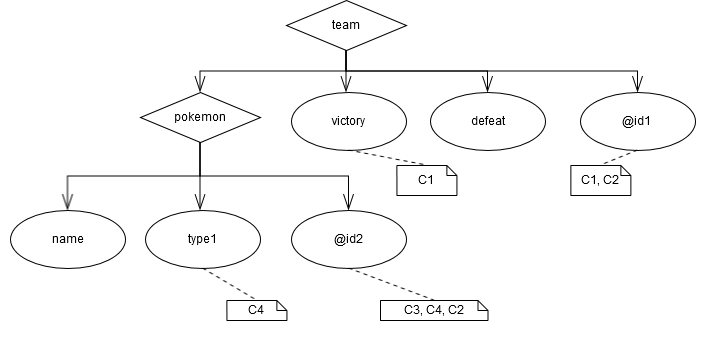
\includegraphics[width=0.8\textwidth]{ressources/graphiques/decision.png}
    \caption{Petite partie du schéma fédéré}
\end{figure}

Dans la première étape, il nous faut relier victory et type1. On utilise un algorithme de décision qui nous donnera la jointure à faire pour relier deux "Clusters" \footnote{un cluster est une table de base ou un fichier xml  comme défini dans notre programme}. Ici on relie C4 et C1. L'algorithme nous donnera la démarche à suivre pour tout relier.


$C1 -id1 \rightarrow C2 -id2 \rightarrow  C4$

En supposant que ces clusters soient tous dans des bases SQL, on fait les deux sous-requêtes suivantes pour joindre victory et type1 :

\begin{lstlisting}
SELECT id1 FROM C1 WHERE victory > 10
SELECT id2 FROM C2 WHERE id2 = id1
\end{lstlisting}

Une fois les sous-requêtes prêtes, elle sont envoyées pour interroger les bases. Des objets sont retournés. Ces objets, pas forcément utiles aux données demandées dans la requête principale, sont réceptionnés, et sont transformés en tant que conditions supplémentaires de la requête principale.

L'attribut intéressant pour réaliser la sélection est extrait. C'est-à-dire : les id2 sont récupérés afin de restreindre type1.

id2 nous a retourné 5 et 6., on produit donc :
\begin{lstlisting}
selection = "id2 = 5 OR id2 = 6"
\end{lstlisting}

Ensuite, on analyse $[. <> "Grass"]$. On le simplifie immédiatement puisqu'il s'agit exactement de l'attribut de retour. L'ultime variable selection est mise à jour:
\begin{lstlisting}
selection = "id2 = 5 OR id2 = 6 OR type <> 'Grass'"
\end{lstlisting}

La requête ultime qui renverra le résultat escompté sera tout simplement :

\begin{lstlisting}
"SELECT type1 FROM C4 WHERE " + selection
\end{lstlisting}

Soit :

\begin{lstlisting}
SELECT type1 FROM C4 WHERE id2 = 5 OR id2 = 6 OR type <> 'Grass'
\end{lstlisting}
En conclusion, grâce à l'arbre représentant le schéma fédéré, nous arrivons a recréer une requete plus simple, touchant à une unique table,  sans avoir à effectuer de joins, la sélection ayant eu lieu plus tôt grâce aux sous-requêtes.

\subsubsection{Wrapper}

Les sous-requêtes sont exprimées dans un langage pivot, compréhensible par tous les "Wrapper" (voir 3) b) ). Les sous-requêtes sont poussées vers les "Wrapper".

Ces derniers reçoivent la requête en langage pivot et commencent par la traduire vers un langage de requête propre à la base, requête SQL pour l'un et requête XQuery pour l'autre. Ils exécutent ensuite la requête auprès de la source de données. Le résultat ainsi produit est ensuite retransformé vers du XML, le langage de retour des "Wrapper". Dans notre cas, l'un des wrappers éxecutant du XQuery, cette transformation est inutile car le résultat est déjà en XML, pour SQL, cependant, cette transformation a bien lieu. Le XML ainsi produit est retourné au "Mediator".

C'est le "Merger" qui continue le traitement de la requête au sein du "Mediator". La particularité des "Wrapper" est d'envoyer au "Merger" le même type de données. Cependant des informations peuvent correspondre au sein de ses données. Le rôle du "Merger" est de traiter ces données apparemment hétérogènes et d'en effectuer les liaisons, lorsque cela est judicieux. Dans notre modèle de données par exemple, les informations propres à une espèce de pokémon sont séparées et se trouvent à la fois dans un fichier XML (ses types) et dans une table SQL (son poids, sa taille, etc.). Lorsque l'utilisateur veut des données générales sur un pokémon donné (donc un "id" donné), le "Merger" devra ici joindre les deux parties de l'information par rapport à l'id. 

\subsection{Architecture et adaptations}

Dans le cadre de notre projet, nous avons décidé d'implémenter une chaîne simple. Les fonctionnalités de chaque niveau (source, médiator et client) sont simplifiées. En effet, il semble plus intéressant de créer une vue d'ensemble pour mieux appréhender une architecture telle que la fédération de bases de données. Ainsi notre application reposera sur la gestion de requêtes simples telle que l'interrogation des bases avec des conditions. En revanche, les mises à jour de bases ne sont pas implémentées car cela augmente grandement la complexité de l'architecture.

\subsubsection{L'architecture globale}

%**** Insérer schéma UML (class\_diagram.eps)****

Présenter l'architecture à l'aide du schéma, et souligner les différences par rapport à ce qui a été présenté dans I.

\subsubsection{Le langage pivot}

Comme évoqué plus haut, le "Splitter" exprime les sous-requêtes, à partir de la requête initiale, dans un langage pivot, que tous les "Wrapper" pourront comprendre et traduire en langage source. Ce langage pivot prend la forme d'un objet python, nommé Req. Cet objet correspond au découpage simple d'une requête en 3 éléments :

\begin{itemize}
    \item le nom des "colonnes" de projection ;
    \item la partie sélection ;
    \item le nom de la table/fichier XML.
\end{itemize}

Un objet Req pourra être instancié de la façon suivante :

\begin{lstlisting}
Req( [ "name", "description"], "@id = 99" "pokemon" )
\end{lstlisting}

C’est donc cet objet qui sera transmis au bon "Wrapper", et qui sera traduit en requête pour la source associée.

Notons que dans le cadre de ce projet, cet objet a été allégé au mieux : il interroge une seule table/un fichier xml de manière simple, à travers une projection, et une sélection. Cette sélection a été limitée à une combinaison, via des AND et des OR, de conditions dont le membre droit est une valeur non-variable. Ainsi, tous les problèmes liés à la fédération, de jointure par exemple, seront traités par le "Mediator", en amont ou en aval.

\subsection{Modules et fichiers}

\subsubsection{"models.py"}

Ce fichier décrit le schéma fédéré, via la fonction schema(), et deux des classes majeures du programme : Req et Cluster. La classe Req décrit l'objet de requête envoyé aux différents aux wrappers et la classe Cluster représente un ensemble "table/fichier" et "wrapper" qui correspond à un objet interrogé.

\subsubsection{"fdb.py"}

Ce fichier est le fichier "main" et est en ce sens le point d'entrée du système.

\subsubsection{"fdb.py"}

Ce fichier comporte une fonction merge qui réalise la "jointure" entre les résultats des sous-requêtes. Cette fonction attend en paramètre un fichier xml qui est lui-même une concaténation des deux fichiers xml à joindre, un XSLT, qui est le XSLT effectuant le merge et le résultat sera stocké dans le troisième paramètre.
